\documentclass[12pt]{article}

% TEMPLATE DEFAULT PACKAGES
\usepackage{amssymb,amsmath,amsfonts,eurosym,geometry,ulem,graphicx,color,setspace,sectsty,comment,natbib,pdflscape,array,adjustbox}

% ADDED PACKAGES FOR THIS MANUSCRIPT
\usepackage{palatino,newtxmath,multirow,titlesec,threeparttable,tabu,booktabs,titlesec,threeparttable,mathtools,bm,bbm,subcaption,pdflscape,tcolorbox,mathrsfs,tikz,graphicx}
% endfloat,

\usepackage{afterpage}
\usepackage[hyphens]{url}
\usepackage[margin=1cm]{caption}

\usepackage[draft]{hyperref}
\newcommand{\tim}{$\,\times\,$}
% FIGURES & TABLES CAPTION STYLING
\captionsetup[figure]{labelfont={bf},name={Figure},labelsep=period}
\captionsetup[table]{labelfont={bf},name={Table},labelsep=period}

% SECTION TITLE SETTINGS
\titlelabel{\thetitle.\enskip}
\titleformat*{\section}{\large\bfseries}
\titleformat*{\subsection}{\normalsize\bfseries}

% COLUMN TYPES
\newcolumntype{L}[1]{>{\raggedright\let\newline\\\arraybackslash\hspace{0pt}}m{#1}}
\newcolumntype{C}{>{\centering\arraybackslash}p{5.2em}}
\newcolumntype{D}{>{\centering\arraybackslash}p{5em}}
\newcolumntype{R}[1]{>{\raggedleft\let\newline\\\arraybackslash\hspace{0pt}}m{#1}}


% MARGINS AND SPACING
\normalem
\geometry{left=1.1in,right=1.1in,top=1.0in,bottom=1.0in}
\setlength{\parskip}{2.5pt}

% SPECIAL CELL 
\newcommand{\specialcell}[2][c]{%
	\begin{tabular}[#1]{@{}l@{}}#2\end{tabular}}

% NO INDENT ON FOOTNOTES
\usepackage[hang,flushmargin]{footmisc}

\begin{document}

\begin{itemize}

    \item \textbf{Greenfield} : 55 Projects labeled ``mixed housing developments'' which according to the Gauteng Department of Housing are basically the new wave of greenfield projects, where community centers, some rental housing, and some better quality housing are mixed in with standard greenfield houses
    \item \textbf{In-Situ Upgrading} : 54 Projects labeled ``essential services'' which from reading Marie Huchemeyer's article follow from a new, aggressive in-situ upgrading initiative complete with bulldozing and replacement of slums that was launched in the mid-2000s in Guateng
    \item \textbf{Other projects} : 198 Projects which I couldn't link any of the descriptions to any clear project definitions; from the results below, the appear to be most like the in-situ projects 
    \item The other new thing is that the density plots now include squares that are empty both before and after projects, which turns out to matter quite a bit, as shown in the plots below

    \item Triple difference specifications are all identical
        \begin{itemize}
            \item no project fixed effects, but clustered at the project level (unless otherwise specified)
            \item ``inside'' project includes all areas within projects
            \item estimate two spillover groups (0-300, and 300-600), which we can adjust later as need be
            \item control distance is 600-1500, which we can also adjust
        \end{itemize}

\end{itemize}




\vspace{0mm}
\begin{table}[h!]
\centering
\caption{Housing Project Areas Description}\label{table:projectdescriptives}
\vspace{0mm}
\begin{tabular}{l*{1}{cccccc}}
\toprule
  & \multicolumn{2}{c}{\textbf{All}}& \multicolumn{2}{c}{\textbf{Greenfield}}  & \multicolumn{2}{c}{\textbf{In-Situ}}   \\
  &Const. & Unconst. &Const. & Unconst.   & Const. & Unconst. \\
\midrule
 Number of Projects  & 172  & 145  & 43  & 20  & 27  & 29  \\ 
 Area (km2)  & 1.17  & 1.16  & 1.72  & 2.42  & 1.50  & 0.88  \\ 
 Median Construction Yr.  & 2006  & 2006  & 2006  & 2005  & 2004  & 2006  \\ 
 Delivered Houses  & 374  & 11  & 568  & 24  & 702  & 20  \\ 
 House Price in 1 km (R$^\dagger$)  & 188,441  & 218,635  & 194,214  & 186,841  & 179,596  & 208,570  \\ 
 Distance to CBD$^\ddagger$ (km)  & 32.5  & 27.7  & 40.5  & 39.9  & 32.6  & 30.6  \\ 

\bottomrule
\multicolumn{7}{l}{\scriptsize Const. refers to constructed projects and unconst. refers to unconstructed projects.}\\[-.5em]
\multicolumn{7}{l}{\scriptsize $^*$Calculated from {\it expected} completion dates using Gauteng National Treasury budget reports.}\\[-.5em]
\multicolumn{7}{l}{\scriptsize $^\dagger$ The USD averaged to about 7.70 Rands during the 2001-2011 period.}\\[-.5em]
\multicolumn{7}{l}{\scriptsize $^\ddagger$Measured as the average minimum distance with respect to Johannesburg and Pretoria CBDs. } \\[-.5em]
%\multicolumn{7}{l}{\scriptsize City includes projects whose centroids are within 30.4 km of their nearest CBD.} \\[-.5em]
%\multicolumn{7}{l}{\scriptsize Suburb includes projects whose centroids are further than 30.4 km from their nearest CBD.}
\end{tabular}
\end{table} 



\begin{table}
\begin{tabular}{lDDDDD}
\toprule
 & \small (1) & \small (2)  & \small (3) & \small (4) & \small (5) \\
 & Total & Formal  & Informal & Informal Bkyd. & Informal Non-Bkyd. \\ \midrule
inside project      &     649.922\textsuperscript{a}&     578.443\textsuperscript{a}&      71.480                   &     504.849\textsuperscript{a}&    -433.370\textsuperscript{a}\\
                    &   (142.583)                   &    (74.803)                   &   (109.399)                   &   (103.801)                   &    (87.272)                   \\[0.55em]
0-300m outside project &      -4.615                   &      34.561                   &     -39.176                   &       6.232                   &     -45.408                   \\
                    &    (43.547)                   &    (24.463)                   &    (35.468)                   &    (31.659)                   &    (28.679)                   \\[0.5em]
300-600m outside project &     -93.284\textsuperscript{b}&      -4.618                   &     -88.666\textsuperscript{a}&     -65.122\textsuperscript{b}&     -23.544                   \\
                    &    (37.619)                   &    (16.266)                   &    (33.159)                   &    (28.282)                   &    (16.891)                   \\[0.5em]
Mean Outcome 2001   &      379.90                   &      203.91                   &      175.98                   &       66.26                   &      109.72                   \\
Mean Outcome 2011   &      584.70                   &      281.66                   &      303.04                   &      192.77                   &      110.27                   \\
R$^2$               &       0.095                   &       0.064                   &       0.079                   &       0.059                   &       0.052                   \\
\# projects         &         308                   &         308                   &         308                   &         308                   &         308                   \\
N project areas     &     266,572                   &     266,572                   &     266,572                   &     266,572                   &     266,572                   \\
N spillover areas   &     501,926                   &     501,926                   &     501,926                   &     501,926                   &     501,926                   \\
N                   &   2,721,910                   &   2,721,910                   &   2,721,910                   &   2,721,910                   &   2,721,910                   \\

\bottomrule
\end{tabular}
\end{table}


\begin{table}
 \resizebox{\linewidth}{!}{
\begin{tabular}{lDDDDD}
\toprule
 & \small (1) & \small (2)  & \small (3) & \small (4) & \small (5) \\
 & Total & Formal  & Informal & Informal Bkyd. & Informal Non-Bkyd. \\ \midrule
\textbf{Greenfield} \\   inside project      &     217.909                   &     222.695\textsuperscript{c}&      -4.785                   &      79.224                   &     -84.009                   \\
                    &   (213.941)                   &   (119.653)                   &   (111.448)                   &   (124.833)                   &    (62.730)                   \\[0.01em]
0-300m outside project &     -44.056                   &       9.956                   &     -54.012                   &     -43.341                   &     -10.671                   \\
                    &    (78.251)                   &    (30.002)                   &    (59.637)                   &    (57.969)                   &    (35.938)                   \\[0.01em]
300-600m outside project&     -81.483\textsuperscript{c}&     -20.464                   &     -61.019\textsuperscript{b}&     -45.399\textsuperscript{c}&     -15.620                   \\
                    &    (46.495)                   &    (26.880)                   &    (30.145)                   &    (23.782)                   &    (19.042)                   \\[0.8em] 
\textbf{In-Situ Upgrading} \\   inside project      &     695.310\textsuperscript{c}&     921.289\textsuperscript{a}&    -225.979                   &     700.269\textsuperscript{b}&    -926.248\textsuperscript{a}\\
                    &   (386.705)                   &   (166.130)                   &   (283.422)                   &   (270.238)                   &   (235.351)                   \\[0.01em]
0-300m outside project &     178.887                   &     200.068\textsuperscript{c}&     -21.180                   &      70.923                   &     -92.103                   \\
                    &   (193.903)                   &   (120.530)                   &   (117.670)                   &   (141.136)                   &    (96.654)                   \\[0.01em]
300-600m outside project &     111.841                   &     176.224\textsuperscript{c}&     -64.383                   &     -32.190                   &     -32.193                   \\
                    &   (141.919)                   &    (94.980)                   &    (85.051)                   &    (97.611)                   &    (70.292)                   \\[0.8em]
\textbf{Other} \\   inside project      &     778.199\textsuperscript{a}&     659.434\textsuperscript{a}&     118.765                   &     615.013\textsuperscript{a}&    -496.249\textsuperscript{a}\\
                    &   (190.566)                   &    (85.015)                   &   (166.248)                   &   (133.791)                   &    (93.505)                   \\[0.01em]
0-300m outside project &    -171.670\textsuperscript{b}&     -24.877                   &    -146.793\textsuperscript{b}&     -37.050                   &    -109.743\textsuperscript{a}\\
                    &    (84.637)                   &    (32.861)                   &    (65.637)                   &    (53.607)                   &    (41.974)                   \\[0.01em]
300-600m outside project &    -220.388\textsuperscript{a}&     -77.165\textsuperscript{a}&    -143.223\textsuperscript{a}&     -82.017\textsuperscript{c}&     -61.206\textsuperscript{b}\\
                    &    (69.087)                   &    (27.133)                   &    (54.004)                   &    (47.646)                   &    (25.964)                   \\[0.8em]
Mean Outcome 2001   &      379.90                   &      203.91                   &      175.98                   &       66.26                   &      109.72                   \\
Mean Outcome 2011   &      584.70                   &      281.66                   &      303.04                   &      192.77                   &      110.27                   \\
R$^2$               &       0.125                   &       0.079                   &       0.106                   &       0.081                   &       0.069                   \\
\# projects         &         308                   &         308                   &         308                   &         308                   &         308                   \\
N project areas     &     266,572                   &     266,572                   &     266,572                   &     266,572                   &     266,572                   \\
N spillover areas   &     501,926                   &     501,926                   &     501,926                   &     501,926                   &     501,926                   \\
N                   &   2,721,910                   &   2,721,910                   &   2,721,910                   &   2,721,910                   &   2,721,910                   \\

\bottomrule
\end{tabular}
}
\end{table}


\afterpage{%
  \clearpage% 
\begin{landscape}
{\footnotesize
\begin{table}[]
\small
\centering
\caption{Census Household-level Estimates}\label{table:censusestimates}
\vspace{-2mm}
\begin{tabular}{lDDDDDDDD}
\toprule
 & \small (1) & \small (2)  & \small (3) & \small (4) & \small (5)  & \small (6)  & \small (7) & (8)\\
 & \small Flush Toilet & \small Water Indoors  & \small Electricity Cooking & \small Electricity Heating & \small Electricity Lighting  & \small Number of Rooms  & \small Household Size & Population Density\\ \midrule 
inside project      &       0.097                   &       0.182\textsuperscript{a}&       0.182\textsuperscript{a}&       0.163\textsuperscript{a}&       0.107                   &       0.069                   &       0.070                   &    -813.497                   \\
                    &     (0.069)                   &     (0.046)                   &     (0.064)                   &     (0.062)                   &     (0.066)                   &     (0.169)                   &     (0.079)                   &  (1228.688)                   \\[0.55em]
0-300m outside project &      -0.042                   &       0.015                   &      -0.015                   &      -0.003                   &      -0.025                   &      -0.092                   &      -0.094\textsuperscript{c}&     385.617                   \\
                    &     (0.036)                   &     (0.038)                   &     (0.034)                   &     (0.036)                   &     (0.032)                   &     (0.119)                   &     (0.054)                   &   (647.578)                   \\[0.5em]
300-600m outside project &      -0.033                   &       0.009                   &      -0.015                   &      -0.001                   &      -0.017                   &      -0.093                   &      -0.048                   &    -247.696                   \\
                    &     (0.027)                   &     (0.033)                   &     (0.027)                   &     (0.029)                   &     (0.026)                   &     (0.109)                   &     (0.052)                   &   (694.350)                   \\[0.5em]
Mean Outcome 2001   &        0.79                   &        0.35                   &        0.66                   &        0.62                   &        0.77                   &        3.30                   &        3.51                   &    8,566.83                   \\
Mean Outcome 2011   &        0.83                   &        0.54                   &        0.81                   &        0.72                   &        0.82                   &        3.56                   &        3.18                   &    9,823.82                   \\
R$^2$               &       0.402                   &       0.414                   &       0.491                   &       0.474                   &       0.442                   &       0.475                   &       0.496                   &       0.458                   \\
\# projects         &         314                   &         314                   &         314                   &         314                   &         314                   &         314                   &         314                   &         314                   \\
N project areas     &       3,657                   &       3,657                   &       3,657                   &       3,657                   &       3,657                   &       3,651                   &       3,657                   &       3,657                   \\
N spillover areas   &       4,200                   &       4,200                   &       4,200                   &       4,200                   &       4,200                   &       4,192                   &       4,199                   &       4,201                   \\
N                   &      12,732                   &      12,732                   &      12,732                   &      12,732                   &      12,732                   &      12,709                   &      12,730                   &      12,734                   \\

\bottomrule
\multicolumn{9}{l}{\footnotesize All regressions include project Fixed-Effects. Standard errors clustered at the project level in parenthesis. \textsuperscript{c} p$<$0.10,\textsuperscript{b} p$<$0.05,\textsuperscript{a} p$<$0.01 }
\end{tabular}
\end{table}
}
\end{landscape}
}

\afterpage{%
  \clearpage% 
\begin{landscape}
{\footnotesize
\begin{table}[]
\small
\centering
\caption{Census Household-level Estimates By Type of Project}\label{table:censusestimates}
\vspace{-2mm}
\begin{tabular}{lDDDDDDDD}
\toprule
 & \small (1) & \small (2)  & \small (3) & \small (4) & \small (5)  & \small (6)  & \small (7) & (8)\\
 & \small Flush Toilet & \small Water Indoors  & \small Electricity Cooking & \small Electricity Heating & \small Electricity Lighting  & \small Number of Rooms  & \small Household Size & Population Density\\ \midrule 
\textbf{Greenfield} \\   inside project      &      -0.033                   &       0.131                   &       0.073                   &       0.035                   &       0.024                   &       0.251                   &       0.200                   &    3790.441\textsuperscript{c}\\
                    &     (0.131)                   &     (0.123)                   &     (0.111)                   &     (0.112)                   &     (0.126)                   &     (0.367)                   &     (0.209)                   &  (2196.802)                   \\[0.01em]
0-300m outside project &      -0.054                   &       0.077                   &       0.014                   &       0.036                   &      -0.030                   &       0.565\textsuperscript{c}&       0.257\textsuperscript{b}&    3716.468                   \\
                    &     (0.089)                   &     (0.091)                   &     (0.060)                   &     (0.069)                   &     (0.057)                   &     (0.287)                   &     (0.125)                   &  (2418.104)                   \\[0.01em]
300-600m outside project&       0.017                   &      -0.025                   &       0.086\textsuperscript{c}&       0.078                   &       0.096\textsuperscript{b}&       0.207                   &       0.126                   &    -466.573                   \\
                    &     (0.060)                   &     (0.076)                   &     (0.044)                   &     (0.059)                   &     (0.042)                   &     (0.195)                   &     (0.102)                   &  (1702.631)                   \\[0.8em] 
\textbf{In-Situ Upgrading} \\   inside project      &       0.320\textsuperscript{a}&       0.217\textsuperscript{b}&       0.347\textsuperscript{a}&       0.379\textsuperscript{a}&       0.220\textsuperscript{b}&       0.322                   &       0.169                   &   -3307.188                   \\
                    &     (0.111)                   &     (0.096)                   &     (0.090)                   &     (0.082)                   &     (0.095)                   &     (0.267)                   &     (0.128)                   &  (3071.103)                   \\[0.01em]
0-300m outside project &       0.018                   &       0.014                   &       0.069                   &       0.093                   &       0.026                   &      -0.250                   &      -0.012                   &    -919.031                   \\
                    &     (0.079)                   &     (0.079)                   &     (0.070)                   &     (0.077)                   &     (0.067)                   &     (0.274)                   &     (0.086)                   &  (1398.915)                   \\[0.01em]
300-600m outside project &      -0.007                   &       0.022                   &       0.051                   &       0.097                   &       0.002                   &      -0.234                   &      -0.083                   &    -269.849                   \\
                    &     (0.064)                   &     (0.074)                   &     (0.068)                   &     (0.072)                   &     (0.056)                   &     (0.301)                   &     (0.088)                   &  (1162.953)                   \\[0.8em]
\textbf{Other} \\   inside project      &      -0.078                   &       0.122\textsuperscript{b}&       0.062                   &       0.020                   &       0.019                   &      -0.302                   &      -0.093                   &    -585.210                   \\
                    &     (0.090)                   &     (0.059)                   &     (0.095)                   &     (0.091)                   &     (0.096)                   &     (0.235)                   &     (0.104)                   &  (1046.339)                   \\[0.01em]
0-300m outside project &      -0.073                   &       0.004                   &      -0.081\textsuperscript{c}&      -0.074\textsuperscript{c}&      -0.060                   &      -0.169                   &      -0.236\textsuperscript{a}&     -51.983                   \\
                    &     (0.045)                   &     (0.053)                   &     (0.045)                   &     (0.044)                   &     (0.043)                   &     (0.149)                   &     (0.078)                   &   (873.961)                   \\[0.01em]
300-600m outside project &      -0.062\textsuperscript{c}&       0.018                   &      -0.071\textsuperscript{c}&      -0.060\textsuperscript{c}&      -0.055                   &      -0.138                   &      -0.121                   &    -338.772                   \\
                    &     (0.033)                   &     (0.046)                   &     (0.036)                   &     (0.035)                   &     (0.035)                   &     (0.136)                   &     (0.076)                   &   (880.842)                   \\[0.8em]
Mean Outcome 2001   &        0.79                   &        0.35                   &        0.66                   &        0.62                   &        0.77                   &        3.30                   &        3.51                   &    8,566.83                   \\
Mean Outcome 2011   &        0.83                   &        0.54                   &        0.81                   &        0.72                   &        0.82                   &        3.56                   &        3.18                   &    9,823.82                   \\
R$^2$               &       0.414                   &       0.425                   &       0.500                   &       0.482                   &       0.450                   &       0.483                   &       0.502                   &       0.463                   \\
\# projects         &         314                   &         314                   &         314                   &         314                   &         314                   &         314                   &         314                   &         314                   \\
N project areas     &       3,657                   &       3,657                   &       3,657                   &       3,657                   &       3,657                   &       3,651                   &       3,657                   &       3,657                   \\
N spillover areas   &       4,200                   &       4,200                   &       4,200                   &       4,200                   &       4,200                   &       4,192                   &       4,199                   &       4,201                   \\
N                   &      12,732                   &      12,732                   &      12,732                   &      12,732                   &      12,732                   &      12,709                   &      12,730                   &      12,734                   \\

\bottomrule
\multicolumn{9}{l}{\footnotesize All regressions include project Fixed-Effects. Standard errors clustered at the project level in parenthesis. \textsuperscript{c} p$<$0.10,\textsuperscript{b} p$<$0.05,\textsuperscript{a} p$<$0.01 }
\end{tabular}
\end{table}
}
\end{landscape}
}







\begin{figure*}
\caption{All Projects}
        %\vspace{2mm}
        \begin{subfigure}[b]{0.495\textwidth}
            \centering
        \caption{Formal}
            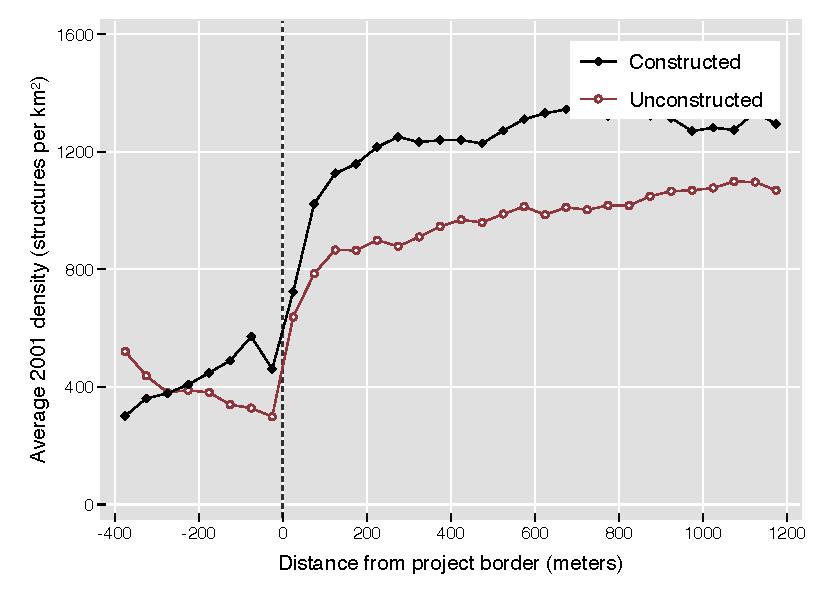
\includegraphics[width=\textwidth,trim={0.3cm .3cm 0.1cm 0cm}, clip=true]{figures/bblu_for_pre_means_4}
        \end{subfigure}
        \hfill
        \begin{subfigure}[b]{0.495\textwidth}  
            \centering 
        \caption{ Informal}
            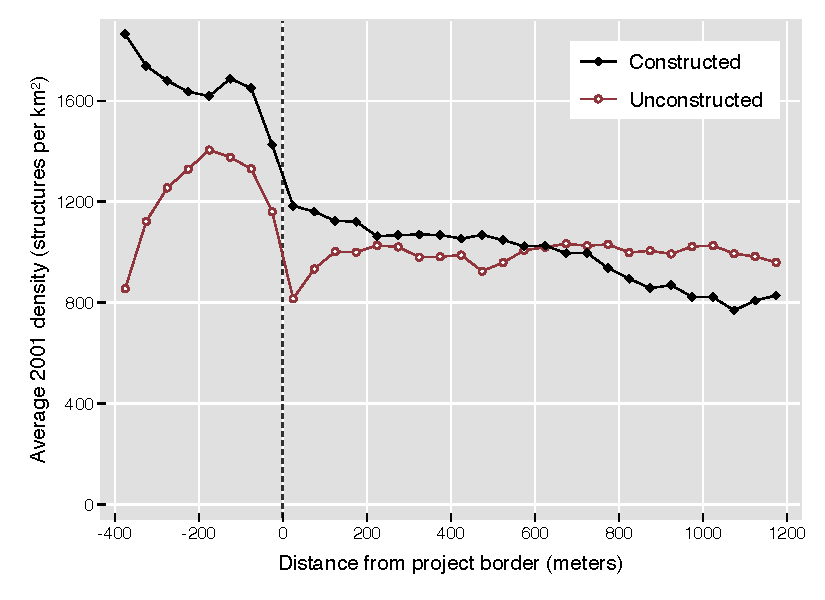
\includegraphics[width=\textwidth,trim={0.3cm .3cm 0.1cm 0cm}, clip=true]{figures/bblu_inf_pre_means_4.pdf}
        \end{subfigure}
        %\vspace{2mm}
        \begin{subfigure}[b]{0.495\textwidth}
            \centering
        \caption{Formal}
            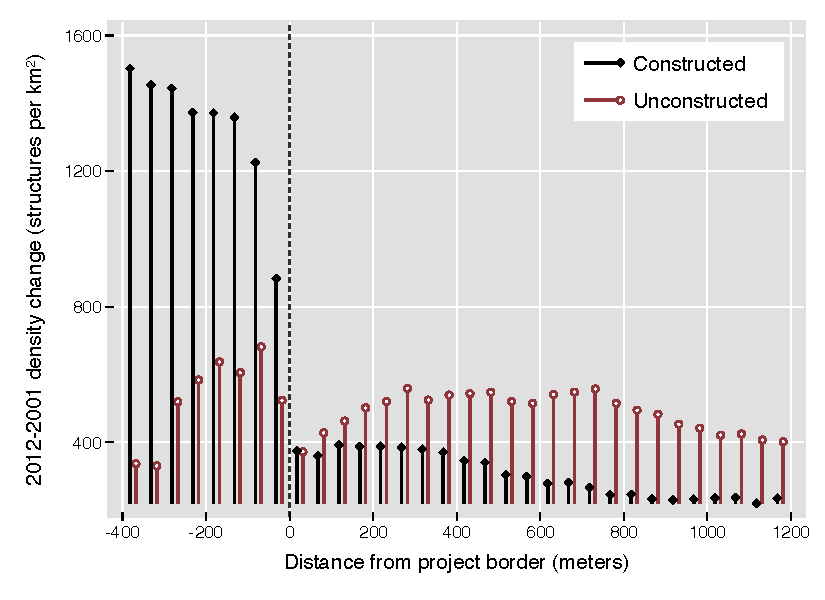
\includegraphics[width=\textwidth,trim={0.3cm .3cm 0.1cm 0cm}, clip=true]{figures/bblu_for_rawchanges_4}
        \end{subfigure}
        \hfill
        \begin{subfigure}[b]{0.495\textwidth}  
            \centering 
        \caption{Informal}
            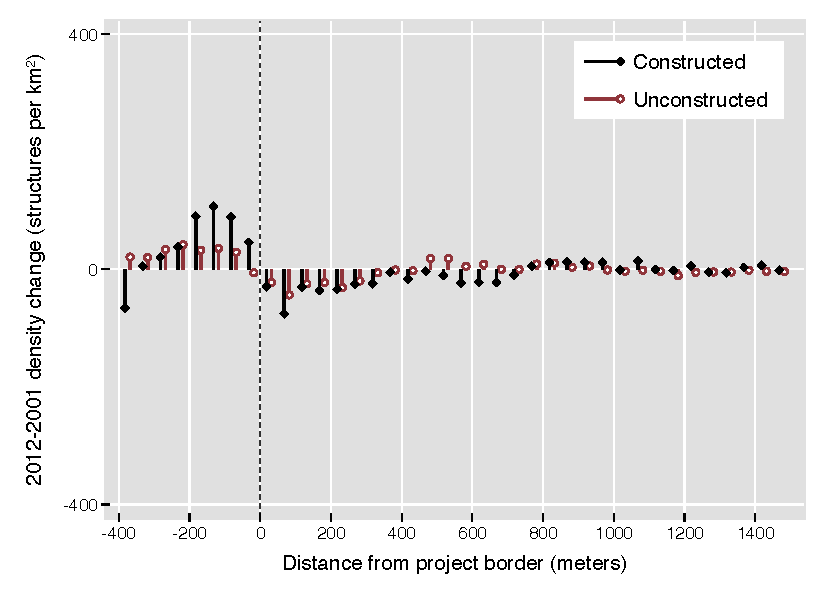
\includegraphics[width=\textwidth,trim={0.3cm .3cm 0.1cm 0cm}, clip=true]{figures/bblu_inf_rawchanges_4.pdf}
        \end{subfigure}
\end{figure*}



\begin{figure*}
\caption{Separately by Project Type}
        %\vspace{2mm}
        \begin{subfigure}[b]{0.495\textwidth}
            \centering
        \caption{Greenfield : Formal}
            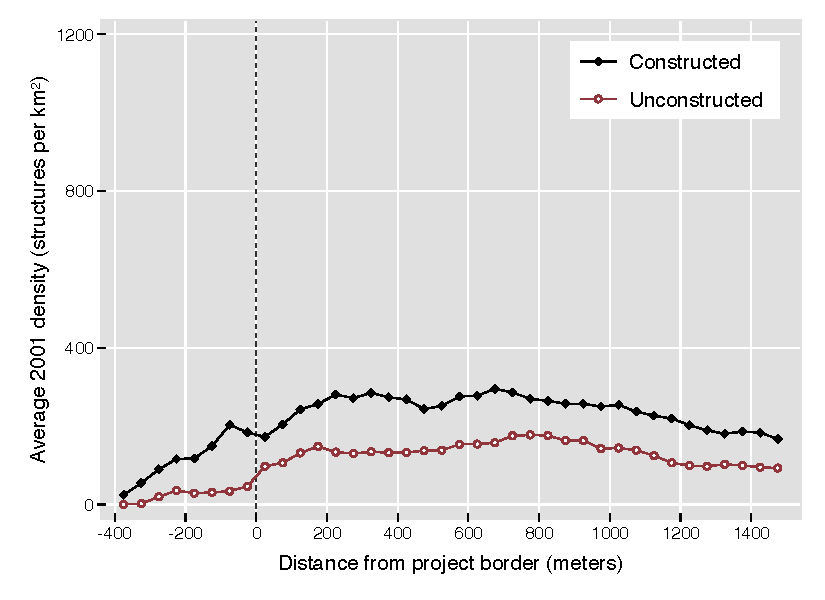
\includegraphics[width=\textwidth,trim={0.3cm .3cm 0.1cm 0cm}, clip=true]{figures/bblu_for_pre_means_4_1}
        \end{subfigure}
        \hfill
        \begin{subfigure}[b]{0.495\textwidth}  
            \centering 
        \caption{Greenfield : Informal}
            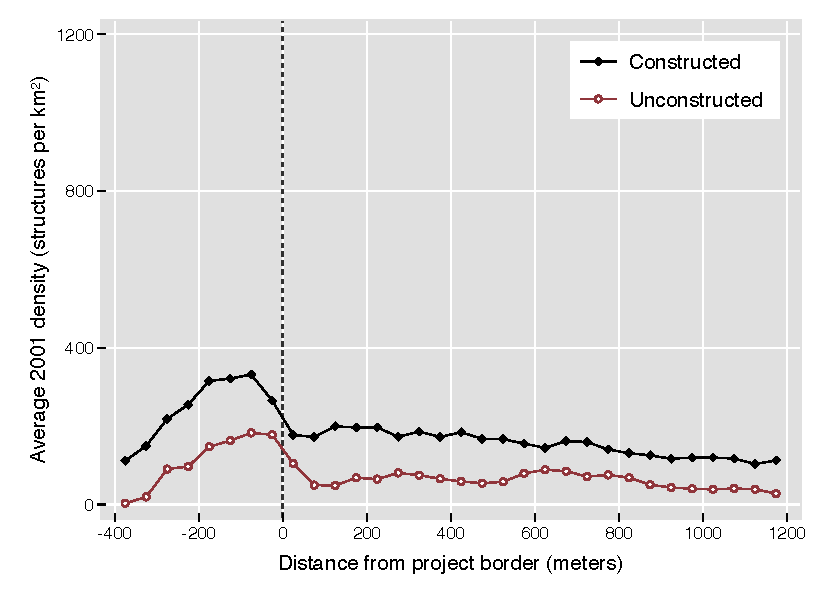
\includegraphics[width=\textwidth,trim={0.3cm .3cm 0.1cm 0cm}, clip=true]{figures/bblu_inf_pre_means_4_1.pdf}
        \end{subfigure}
        %\vspace{-6mm}
        %\vspace{2mm}
        \begin{subfigure}[b]{0.495\textwidth}
            \centering
        \caption{In-Situ Upgrading : Formal}
            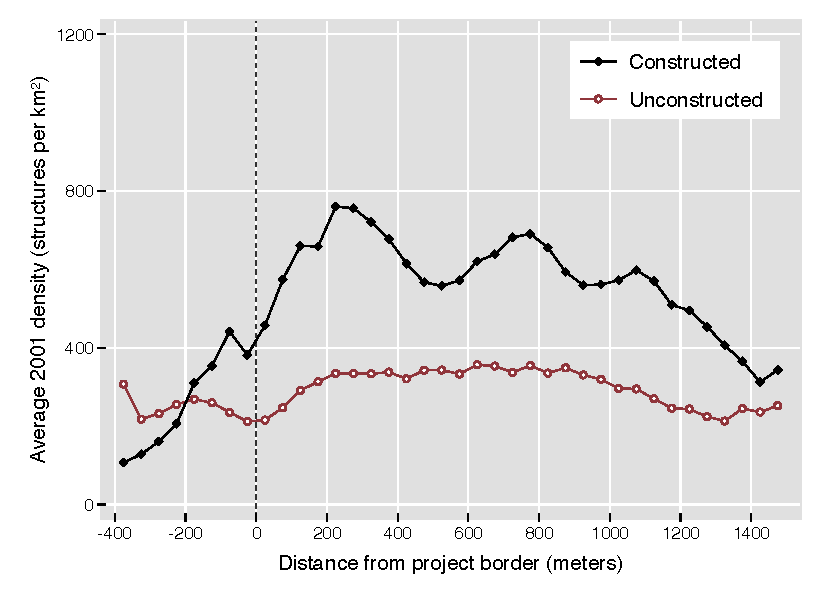
\includegraphics[width=\textwidth,trim={0.3cm .3cm 0.1cm 0cm}, clip=true]{figures/bblu_for_pre_means_4_2.pdf}
        \end{subfigure}
        \hfill
        %\vspace{2mm}
        \begin{subfigure}[b]{0.495\textwidth}
            \centering
        \caption{In-Situ Upgrading : Informal}
                %        Mixed Dev
            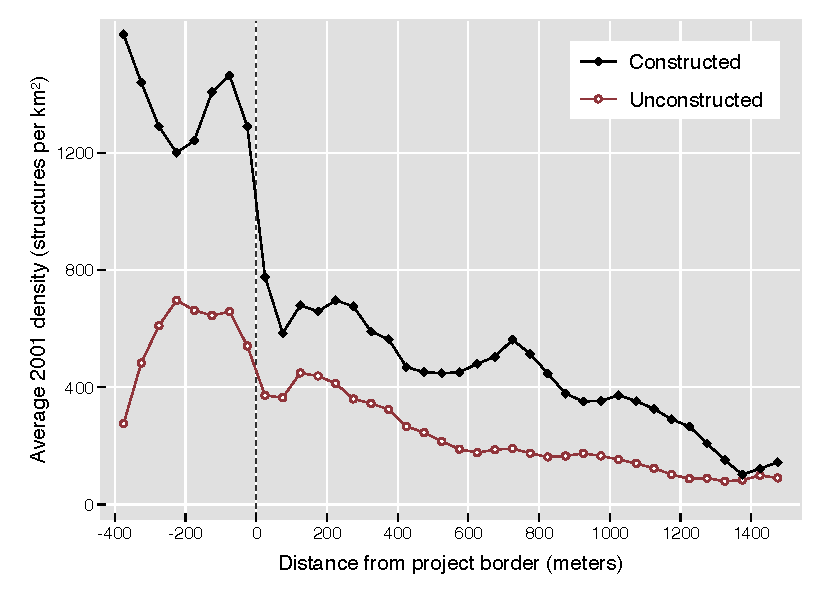
\includegraphics[width=\textwidth,trim={0.3cm .3cm 0.1cm 0cm}, clip=true]{figures/bblu_inf_pre_means_4_2.pdf}
        \end{subfigure}
                %\vspace{2mm}
        %\vspace{-6mm}
        \begin{subfigure}[b]{0.495\textwidth}  
            \centering 
            \caption{Other : Formal}
                %        Essential
            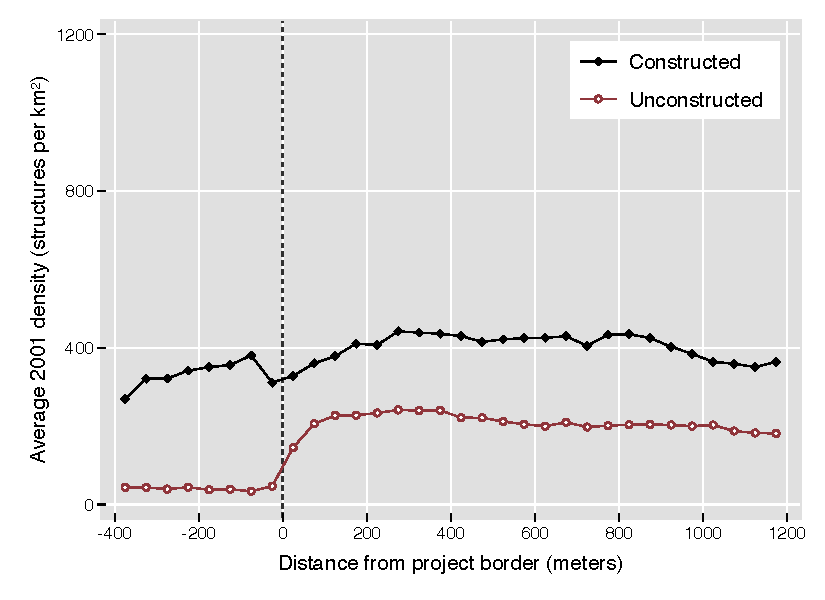
\includegraphics[width=\textwidth,trim={0.3cm .3cm 0.1cm 0cm}, clip=true]{figures/bblu_for_pre_means_4_3.pdf}
        \end{subfigure}
        \hfill
        %\vspace{2mm}
        \begin{subfigure}[b]{0.495\textwidth}
            \centering
            \caption{Other : Informal}
                  %      GDOH
            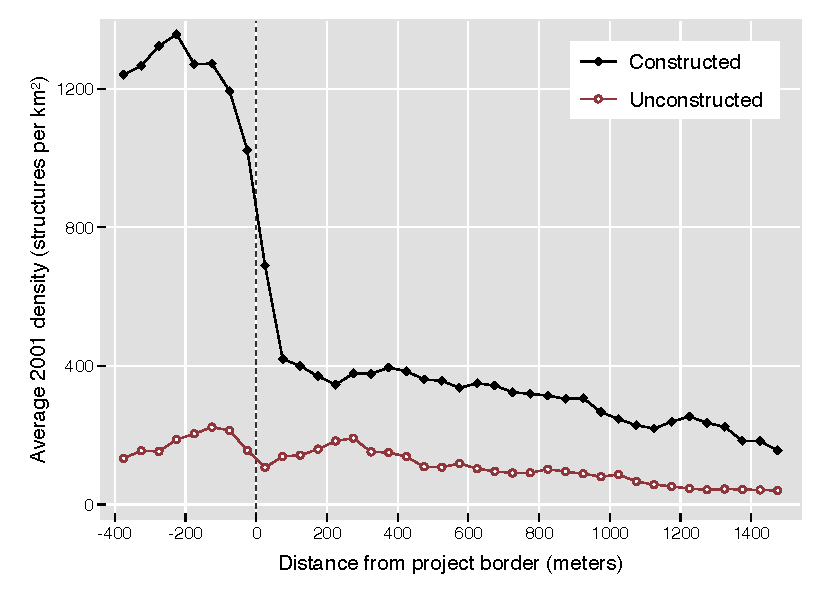
\includegraphics[width=\textwidth,trim={0.3cm .3cm 0.1cm 0cm}, clip=true]{figures/bblu_inf_pre_means_4_3.pdf}
        \end{subfigure}
        % \hfill
        % \begin{subfigure}[b]{0.495\textwidth}  
        %     \centering 
        %            %     Other
        %     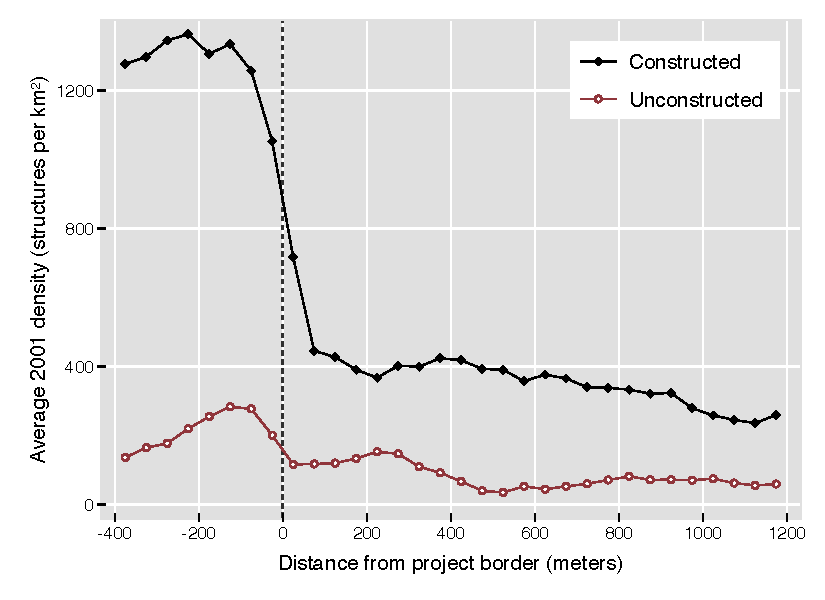
\includegraphics[width=\textwidth,trim={0.3cm .3cm 0.1cm 0cm}, clip=true]{figures/bblu_inf_pre_means_4_4.pdf}
        % \end{subfigure}
        % \vspace{-6mm}
    \end{figure*} 




\begin{figure*}
\caption{Separately by Project Type}
        %\vspace{2mm}
        \begin{subfigure}[b]{0.495\textwidth}
            \centering
        \caption{Greenfield : Formal}
            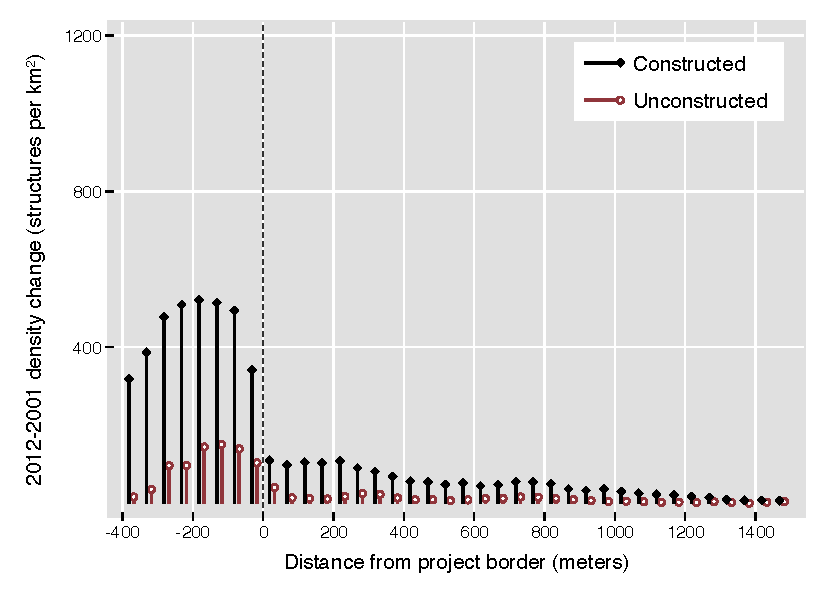
\includegraphics[width=\textwidth,trim={0.3cm .3cm 0.1cm 0cm}, clip=true]{figures/bblu_for_rawchanges_4_1}
        \end{subfigure}
        \hfill
        \begin{subfigure}[b]{0.495\textwidth}  
            \centering 
        \caption{Greenfield : Informal}
            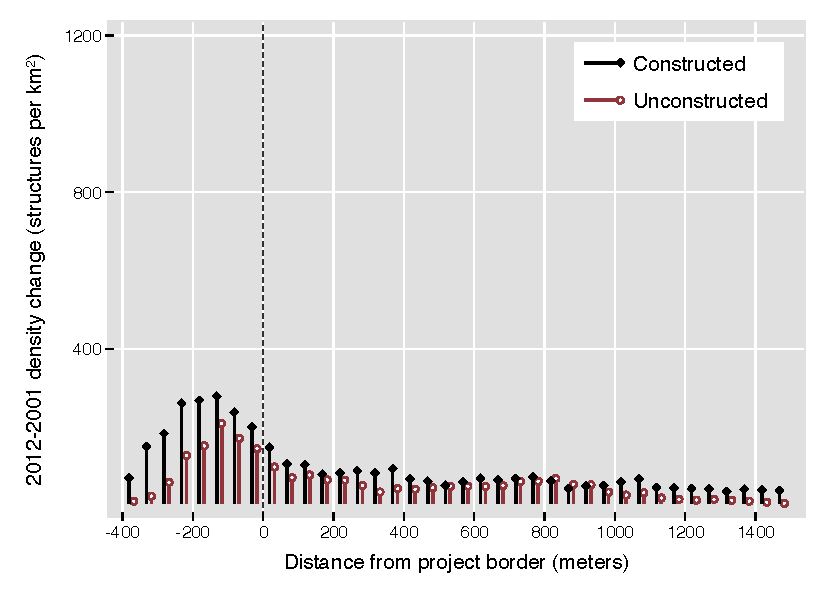
\includegraphics[width=\textwidth,trim={0.3cm .3cm 0.1cm 0cm}, clip=true]{figures/bblu_inf_rawchanges_4_1.pdf}
        \end{subfigure}
        %\vspace{-6mm}
        %\vspace{2mm}
        \begin{subfigure}[b]{0.495\textwidth}
            \centering
        \caption{In-Situ Upgrading : Formal}
            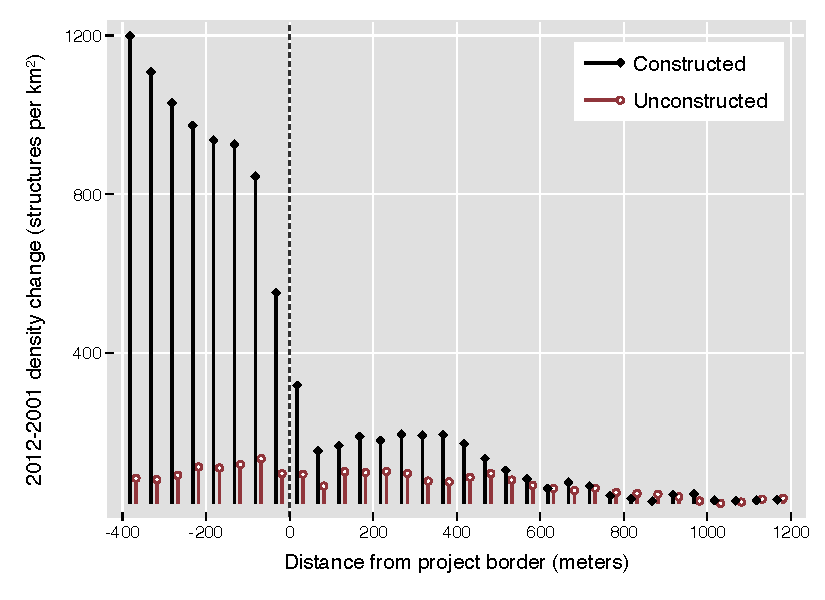
\includegraphics[width=\textwidth,trim={0.3cm .3cm 0.1cm 0cm}, clip=true]{figures/bblu_for_rawchanges_4_2.pdf}
        \end{subfigure}
        \hfill
        %\vspace{2mm}
        \begin{subfigure}[b]{0.495\textwidth}
            \centering
        \caption{In-Situ Upgrading : Informal}
                %        Mixed Dev
            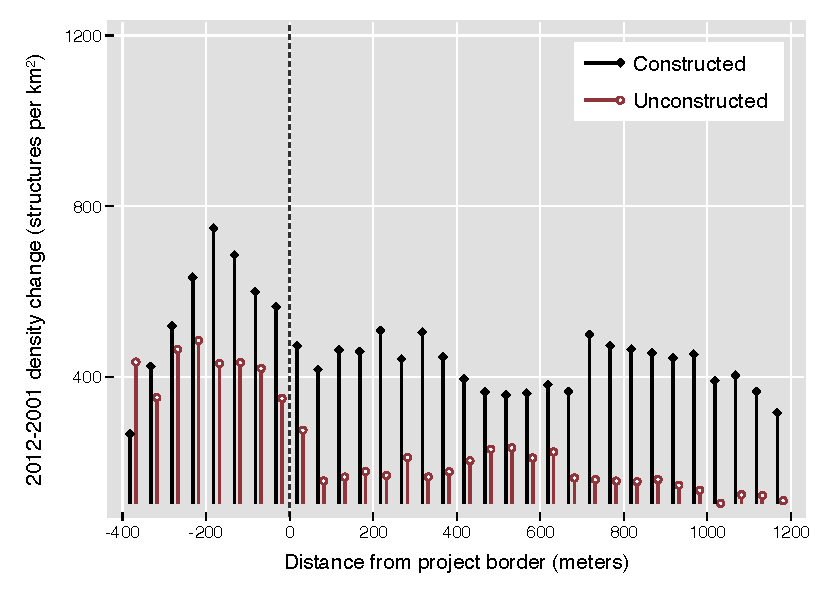
\includegraphics[width=\textwidth,trim={0.3cm .3cm 0.1cm 0cm}, clip=true]{figures/bblu_inf_rawchanges_4_2.pdf}
        \end{subfigure}
                %\vspace{2mm}
        %\vspace{-6mm}
        \begin{subfigure}[b]{0.495\textwidth}  
            \centering 
            \caption{Other : Formal}
                %        Essential
            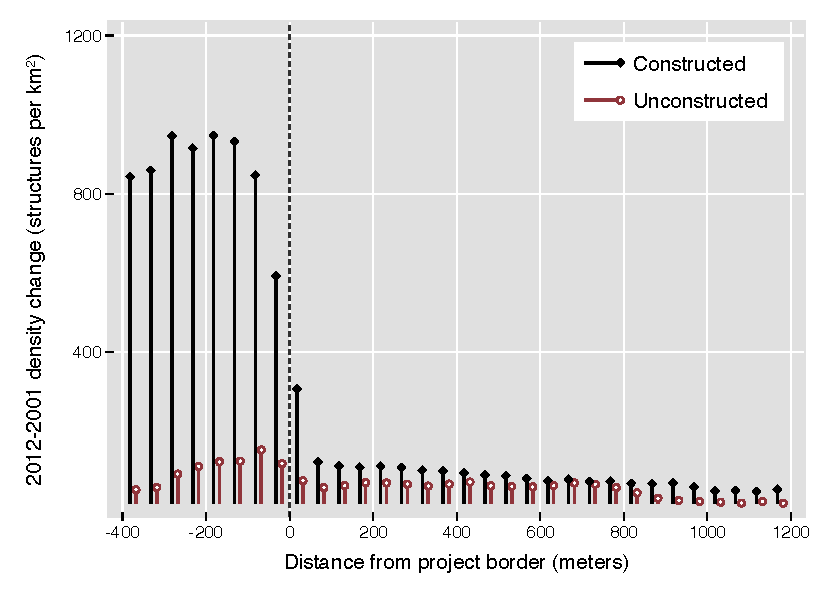
\includegraphics[width=\textwidth,trim={0.3cm .3cm 0.1cm 0cm}, clip=true]{figures/bblu_for_rawchanges_4_3.pdf}
        \end{subfigure}
        \hfill
        %\vspace{2mm}
        \begin{subfigure}[b]{0.495\textwidth}
            \centering
            \caption{Other : Informal}
                  %      GDOH
            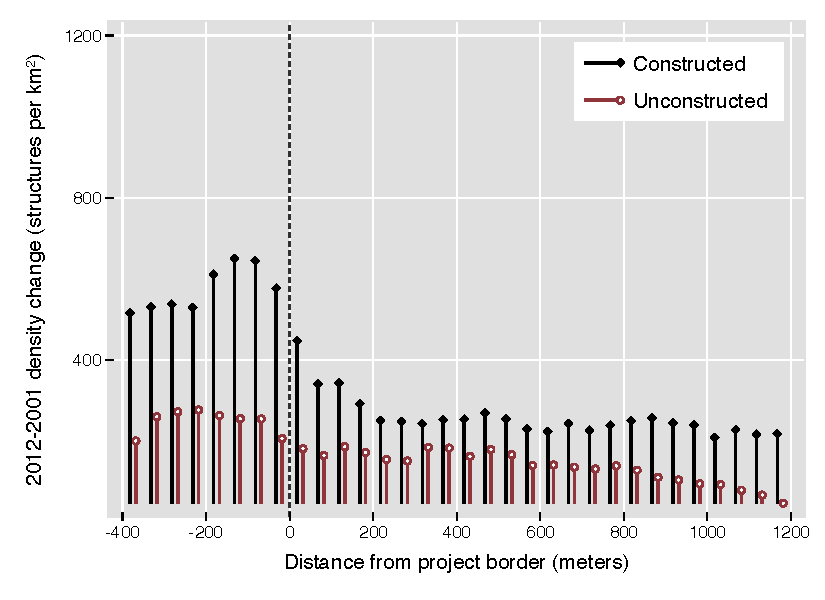
\includegraphics[width=\textwidth,trim={0.3cm .3cm 0.1cm 0cm}, clip=true]{figures/bblu_inf_rawchanges_4_3.pdf}
        \end{subfigure}
        % \hfill
        % \begin{subfigure}[b]{0.495\textwidth}  
        %     \centering 
        %            %     Other
        %     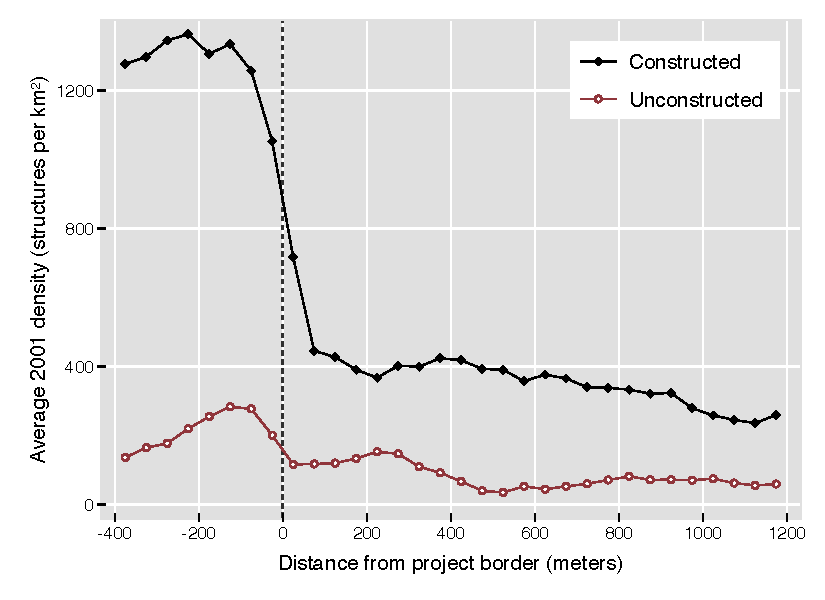
\includegraphics[width=\textwidth,trim={0.3cm .3cm 0.1cm 0cm}, clip=true]{figures/bblu_inf_pre_means_4_4.pdf}
        % \end{subfigure}
        % \vspace{-6mm}
    \end{figure*} 


\begin{table}[h!] 
\caption{Effect of Housing Projects on Socio-demographics}
\label{table:sorting}
\small
\centering
%\caption{Census Composition Estimates }
\vspace{-2mm}
\begin{tabular}{lDDDDD}
\toprule
& \small (1) & \small (2) & \small (3) & \small (4)& \small (5)\\
& \small Age & \small P.O.B. not Gauteng & \small Unemployed & \small Years of Education & \small Monthly Income \\ \midrule 
inside project      &       0.112                   &      -0.029                   &      -0.008                   &       0.165                   &     333.092                   \\
                    &     (0.298)                   &     (0.021)                   &     (0.021)                   &     (0.158)                   &   (553.256)                   \\[0.55em]
0-300m outside project &       0.425                   &       0.021                   &       0.009                   &       0.078                   &     -78.108                   \\
                    &     (0.285)                   &     (0.016)                   &     (0.016)                   &     (0.115)                   &   (524.996)                   \\[0.5em]
300-600m outside project &       0.045                   &       0.011                   &       0.019                   &       0.095                   &      91.017                   \\
                    &     (0.304)                   &     (0.016)                   &     (0.016)                   &     (0.103)                   &   (459.385)                   \\[0.5em]
Mean Outcome 2001   &       27.31                   &        0.37                   &        0.47                   &        8.27                   &    2,480.46                   \\
Mean Outcome 2011   &       28.29                   &        0.43                   &        0.33                   &        9.68                   &    4,506.34                   \\
R$^2$               &       0.513                   &       0.614                   &       0.419                   &       0.584                   &       0.539                   \\
\# projects         &         314                   &         314                   &         314                   &         314                   &         314                   \\
N project areas     &       3,656                   &       3,656                   &       3,656                   &       3,656                   &       3,656                   \\
N spillover areas   &       4,201                   &       4,198                   &       4,196                   &       4,198                   &       4,196                   \\
N                   &      12,733                   &      12,728                   &      12,725                   &      12,728                   &      12,724                   \\

\bottomrule
\multicolumn{6}{l}{\footnotesize Standard errors clustered at the project level in parenthesis. \textsuperscript{c} p$<$0.10, \textsuperscript{b} p$<$0.05, \textsuperscript{a} p$<$0.01  }\\
\multicolumn{6}{l}{\footnotesize P.O.B. means ``place of birth.''  Monthly income is in Rands.}
\end{tabular}
\end{table}




\begin{table}[h!] 
\caption{Effect of Housing Projects on Socio-demographics by Type}
\label{table:sorting}
\small
\centering
%\caption{Census Composition Estimates }
\vspace{-2mm}
\begin{tabular}{lDDDDD}
\toprule
& \small (1) & \small (2) & \small (3) & \small (4)& \small (5)\\
& \small Age & \small P.O.B. not Gauteng & \small Unemployed & \small Years of Education & \small Monthly Income \\ \midrule 
\textbf{Greenfield} \\   inside project      &      -1.409\textsuperscript{c}&      -0.048                   &       0.140\textsuperscript{a}&      -1.165\textsuperscript{b}&   -1486.342\textsuperscript{c}\\
                    &     (0.749)                   &     (0.052)                   &     (0.051)                   &     (0.451)                   &   (855.477)                   \\[0.01em]
0-300m outside project &      -0.906                   &      -0.100\textsuperscript{b}&       0.139\textsuperscript{a}&      -0.774\textsuperscript{b}&   -1189.553                   \\
                    &     (0.718)                   &     (0.044)                   &     (0.047)                   &     (0.365)                   &  (1030.247)                   \\[0.01em]
300-600m outside project&      -0.874                   &      -0.058                   &       0.043                   &      -0.134                   &    -974.465                   \\
                    &     (0.905)                   &     (0.046)                   &     (0.057)                   &     (0.344)                   &  (1156.804)                   \\[0.8em] 
\textbf{In-Situ Upgrading} \\   inside project      &       0.434                   &      -0.119\textsuperscript{c}&       0.017                   &       0.321                   &    1488.620                   \\
                    &     (0.907)                   &     (0.065)                   &     (0.035)                   &     (0.250)                   &  (1572.224)                   \\[0.01em]
0-300m outside project &      -0.246                   &      -0.036                   &       0.025                   &       0.442                   &    1706.076                   \\
                    &     (0.870)                   &     (0.058)                   &     (0.042)                   &     (0.277)                   &  (1579.078)                   \\[0.01em]
300-600m outside project &      -0.775                   &      -0.004                   &       0.034                   &      -0.007                   &    -593.232                   \\
                    &     (0.920)                   &     (0.052)                   &     (0.037)                   &     (0.271)                   &  (1370.201)                   \\[0.8em]
\textbf{Other} \\   inside project      &       0.564                   &       0.014                   &      -0.013                   &       0.585\textsuperscript{a}&    2971.996\textsuperscript{a}\\
                    &     (0.557)                   &     (0.041)                   &     (0.032)                   &     (0.209)                   &   (960.085)                   \\[0.01em]
0-300m outside project &       1.158\textsuperscript{c}&       0.069\textsuperscript{c}&      -0.015                   &       0.163                   &    1048.665                   \\
                    &     (0.597)                   &     (0.037)                   &     (0.029)                   &     (0.161)                   &   (831.451)                   \\[0.01em]
300-600m outside project &       0.593                   &       0.023                   &      -0.001                   &       0.093                   &    1389.669\textsuperscript{c}\\
                    &     (0.556)                   &     (0.034)                   &     (0.028)                   &     (0.169)                   &   (746.539)                   \\[0.8em]
Mean Outcome 2001   &       27.30                   &        0.37                   &        0.47                   &        8.27                   &    2,482.85                   \\
Mean Outcome 2011   &       28.29                   &        0.43                   &        0.33                   &        9.68                   &    4,512.03                   \\
R$^2$               &       0.201                   &       0.154                   &       0.206                   &       0.395                   &       0.185                   \\
\# projects         &         314                   &         314                   &         314                   &         314                   &         314                   \\
N project areas     &       3,656                   &       3,655                   &       3,655                   &       3,655                   &       3,654                   \\
N spillover areas   &       4,201                   &       4,197                   &       4,196                   &       4,197                   &       4,195                   \\
N                   &      12,733                   &      12,726                   &      12,725                   &      12,726                   &      12,722                   \\

\bottomrule
\multicolumn{6}{l}{\footnotesize Standard errors clustered at the project level in parenthesis. \textsuperscript{c} p$<$0.10, \textsuperscript{b} p$<$0.05, \textsuperscript{a} p$<$0.01  }\\
\multicolumn{6}{l}{\footnotesize P.O.B. means ``place of birth.''  Monthly income is in Rands.}
\end{tabular}
\end{table}


\begin{table}
\small
\centering
\caption{Triple Difference Estimates on Log-Prices}\label{table:priceDDD_het}
\vspace{-2mm}
\begin{tabular}{lCCCC}
\toprule
 & \small (1) & \small (2) & \small (3) & \small (4) \\ \midrule 
inside project      &       0.297                   &      -0.210                   &      -0.223                   &      -0.403                   \\
                    &     (0.536)                   &     (0.322)                   &     (0.312)                   &     (0.458)                   \\[0.55em]
0-300m outside project &      -0.218                   &      -0.229                   &      -0.182                   &      -0.210                   \\
                    &     (0.174)                   &     (0.154)                   &     (0.167)                   &     (0.144)                   \\[0.5em]
300-600m outside project &      -0.118                   &      -0.166                   &      -0.123                   &      -0.170\textsuperscript{c}\\
                    &     (0.135)                   &     (0.107)                   &     (0.111)                   &     (0.092)                   \\[0.5em]
Cluster FE          &                               &  \checkmark                   &                               &                               \\
Cluster {\tim} Year FE&                               &                               &  \checkmark                   &                               \\
Lat.-Long. {\tim} Year FE&                               &                               &                               &  \checkmark                   \\
r2                  &        0.18                   &        0.37                   &        0.41                   &        0.27                   \\
N                   &      67,751                   &      67,751                   &      67,751                   &      67,751                   \\

\bottomrule
\multicolumn{5}{l}{\footnotesize Standard errors clustered at the project level in parenthesis. \textsuperscript{c} p$<$0.10,\textsuperscript{b} p$<$0.05,\textsuperscript{a} p$<$0.01 }
\end{tabular}
\end{table} 


\begin{table}
\small
\centering
\caption{Triple Difference Estimates on Log-Prices by Project Type}\label{table:priceDDD_het}
\vspace{-2mm}
\begin{tabular}{lCCCC}
\toprule
 & \small (1) & \small (2) & \small (3) & \small (4) \\ \midrule 
\textbf{Greenfield} \\   inside project      &      -0.031                   &      -0.087                   &      -0.192                   &      -0.353                   \\
                    &     (0.432)                   &     (0.354)                   &     (0.358)                   &     (0.657)                   \\[0.01em]
0-300m outside project &      -0.142                   &       0.164                   &       0.088                   &      -0.265                   \\
                    &     (0.343)                   &     (0.233)                   &     (0.264)                   &     (0.281)                   \\[0.01em]
300-600m outside project&      -0.184                   &      -0.004                   &      -0.038                   &      -0.272                   \\
                    &     (0.290)                   &     (0.206)                   &     (0.226)                   &     (0.304)                   \\[0.8em]
\textbf{In-Situ Upgrading} \\   inside project      &       0.351                   &       0.299                   &       0.165                   &      -0.139                   \\
                    &     (0.573)                   &     (0.488)                   &     (0.487)                   &     (0.675)                   \\[0.01em]
0-300m outside project &      -0.151                   &      -0.282                   &      -0.244                   &      -0.314                   \\
                    &     (0.398)                   &     (0.367)                   &     (0.384)                   &     (0.315)                   \\[0.01em]
300-600m outside project &      -0.225                   &      -0.203                   &      -0.209                   &      -0.353\textsuperscript{c}\\
                    &     (0.231)                   &     (0.258)                   &     (0.271)                   &     (0.198)                   \\[0.8em]
\textbf{Other} \\   inside project      &      -0.039                   &      -0.390                   &      -0.379                   &      -0.506                   \\
                    &     (0.579)                   &     (0.417)                   &     (0.422)                   &     (0.517)                   \\[0.01em]
0-300m outside project &      -0.237                   &      -0.275\textsuperscript{b}&      -0.198                   &      -0.251                   \\
                    &     (0.215)                   &     (0.138)                   &     (0.158)                   &     (0.167)                   \\[0.01em]
300-600m outside project &      -0.086                   &      -0.200\textsuperscript{c}&      -0.111                   &      -0.160                   \\
                    &     (0.176)                   &     (0.108)                   &     (0.113)                   &     (0.143)                   \\[0.8em]
Cluster FE          &                               &  \checkmark                   &                               &                               \\
Cluster {\tim} Year FE&                               &                               &  \checkmark                   &                               \\
Lat.-Long. {\tim} Year FE&                               &                               &                               &  \checkmark                   \\
r2                  &        0.21                   &        0.37                   &        0.41                   &        0.28                   \\
N                   &      67,751                   &      67,751                   &      67,751                   &      67,751                   \\

\bottomrule
\multicolumn{5}{l}{\footnotesize Standard errors clustered at the project level in parenthesis. \textsuperscript{c} p$<$0.10,\textsuperscript{b} p$<$0.05,\textsuperscript{a} p$<$0.01 }
\end{tabular}
\end{table} 


\begin{figure}
\caption{Triple Difference Price effects over time and distance}
\centering
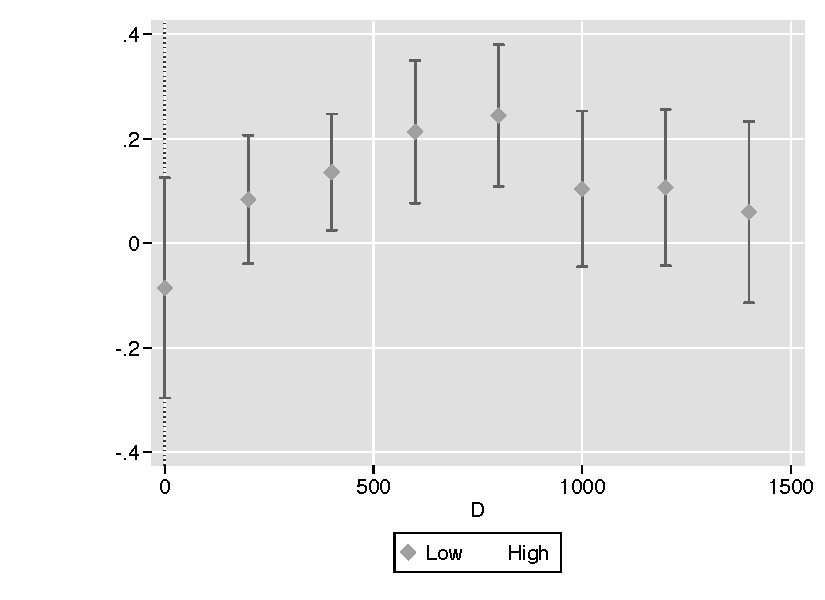
\includegraphics[scale=.7]{figures/price_to_event.pdf}

\end{figure}

\section{My quick interpretation}
\begin{itemize}
\item Buildings
\begin{itemize}
    \item within proj footprints: huge increase in formal structures across all types,  most massive increases are in in-situ/other with more modest increases in greenfield; substitution away from non-bkyd to bkyd informal, some decline in total informal for in-situ/other projects
    \item outside proj footprints: overall little net change, some crowding out of informal (maybe some growth in formal); in-situ seems to crowd in formal housing while other projects seem to crowd out informal housing
\end{itemize}
\item HH Census
\begin{itemize}
    \item within proj footprints: huge improvements in housing quality for insitu-upgrading, more mixed results/declines in quality for greenfield and other projects
    \item outside proj footprints: close to zero net change in quality; some gains in service quality for in-situ upgrading projects with decreases for greenfield and other projects (pretty much matches the building results)
    \item noisy decrease in pop density both within and around projects
\end{itemize}
\item Person Census
\begin{itemize}
    \item within proj footprints: greenfields attract younger, unemployed, less educated poorer people; in-situ and other attract slightly older, same edu, maybe a little richer people
    \item outside proj footprints: greenfields again attract younger, poorer, less educated people; evidence is more mixed for in-situ and other
\end{itemize}

\item Prices
\begin{itemize}
    \item unanimous price declines for all project types, distances, and controls; the effects attenuate somewhat with distance, they aren't very statistically significant
    \item note: I include a few non-project houses within footprints to keep all specifications the same (can also remove later)
\end{itemize}

\item Tentative Conclusion:
\begin{itemize}
    \item large increases in the total supply of housing and large improvements in housing quality within projects are not enough to crowd in substantial housing investments in areas around projects; instead, this housing supply increase may put downward pressure on local housing prices
%    \item housing prices adjust downward, preventing 
\end{itemize}

\end{itemize}

\end{document}


